%%%%%%%%%%%%%%%%%%%%%%%%%%%%%%%%%%%%%%%%%%%%%%%%%%%%%%%%%%%%%%%%%%%%%%%%%%%%%%%%%%%%%%%%%%%%%%
%%%%%%%%%%%%%%%%%%%%%%%%%%%%%%%%%%%%%%%%%%%%%%%%%%%%%%%%%%%%%%%%%%%%%%%%%%%%%%%%%%%%%%%%%%%%%%
%%%%%%%%%%% systemOverview
%%%%%%%%%%%%%%%%%%%%%%%%%%%%%%%%%%%%%%%%%%%%%%%%%%%%%%%%%%%%%%%%%%%%%%%%%%%%%%%%%%%%%%%%%%%%%%
%%%%%%%%%%%%%%%%%%%%%%%%%%%%%%%%%%%%%%%%%%%%%%%%%%%%%%%%%%%%%%%%%%%%%%%%%%%%%%%%%%%%%%%%%%%%%%


% \cleardoublepage
\chapter{System Overview}
\label{sec:systemOverview}






\begin{figure}
	\centering
\includegraphics[width=11.25in/100*55]{figures/systemOverview/ComputationalFlowBlock.pdf}
	\label{fig:ComputationalFlowBlock}
		\caption{Computational Flow Block Diagram.}
\end{figure}
\clearpage
\begin{sidewaysfigure}
	\centering
\includegraphics[width=12.89in/100*55]{figures/systemOverview/ProcessingBlock_new.pdf}
	\label{fig:ProcessingBlock_new}
	\caption{Processing Block Diagram.}
\end{sidewaysfigure}
\begin{figure}
	\centering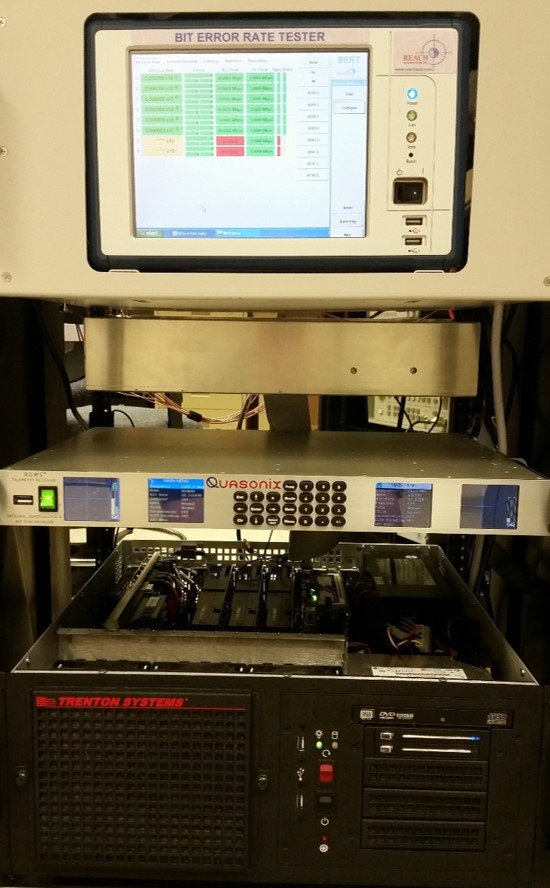
\includegraphics[scale=1]{figures/systemOverview/FullSystem.jpg}
	\label{fig:FullSystem}
	\caption{Picture of full System.}
\end{figure}

\begin{figure}
	\centering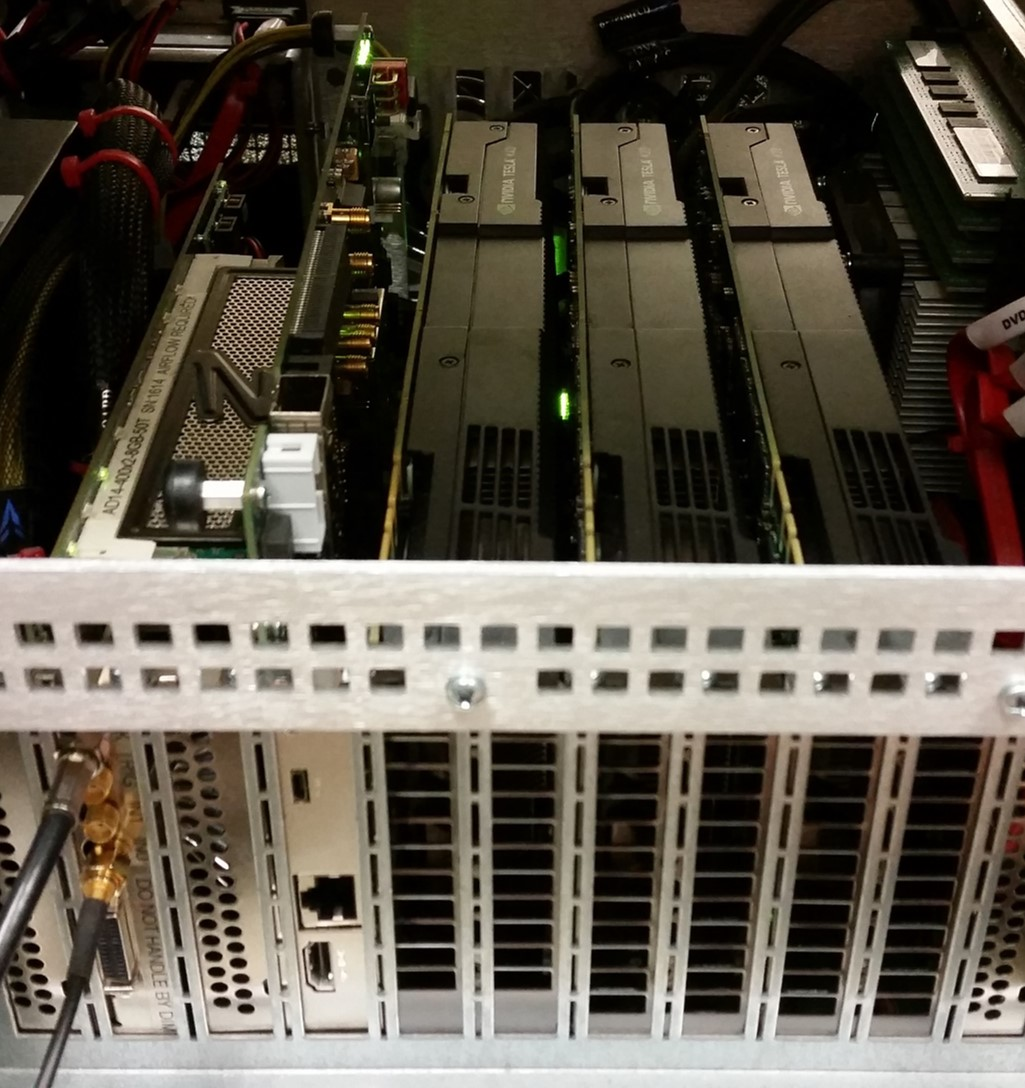
\includegraphics[scale=0.5]{figures/systemOverview/HostSystem.jpg}
	\label{fig:HostSystem}
	\caption{Picture of Processing MIGHT!}
\end{figure}
%The PAQ system is suited very well for batched processing.
%Each $1.907$ second set has $3104$ packets or batches of data as shown in Figure \ref{fig:packet_batch_set}.
%If an operation is done on each packet, available CUDA batched libraries should always be used.
%For simplicity, every block diagram shown in this chapter only applies to a single batch.
%Every block diagram is batched and applied to $3104$ iNET packets.
\begin{figure}
	\centering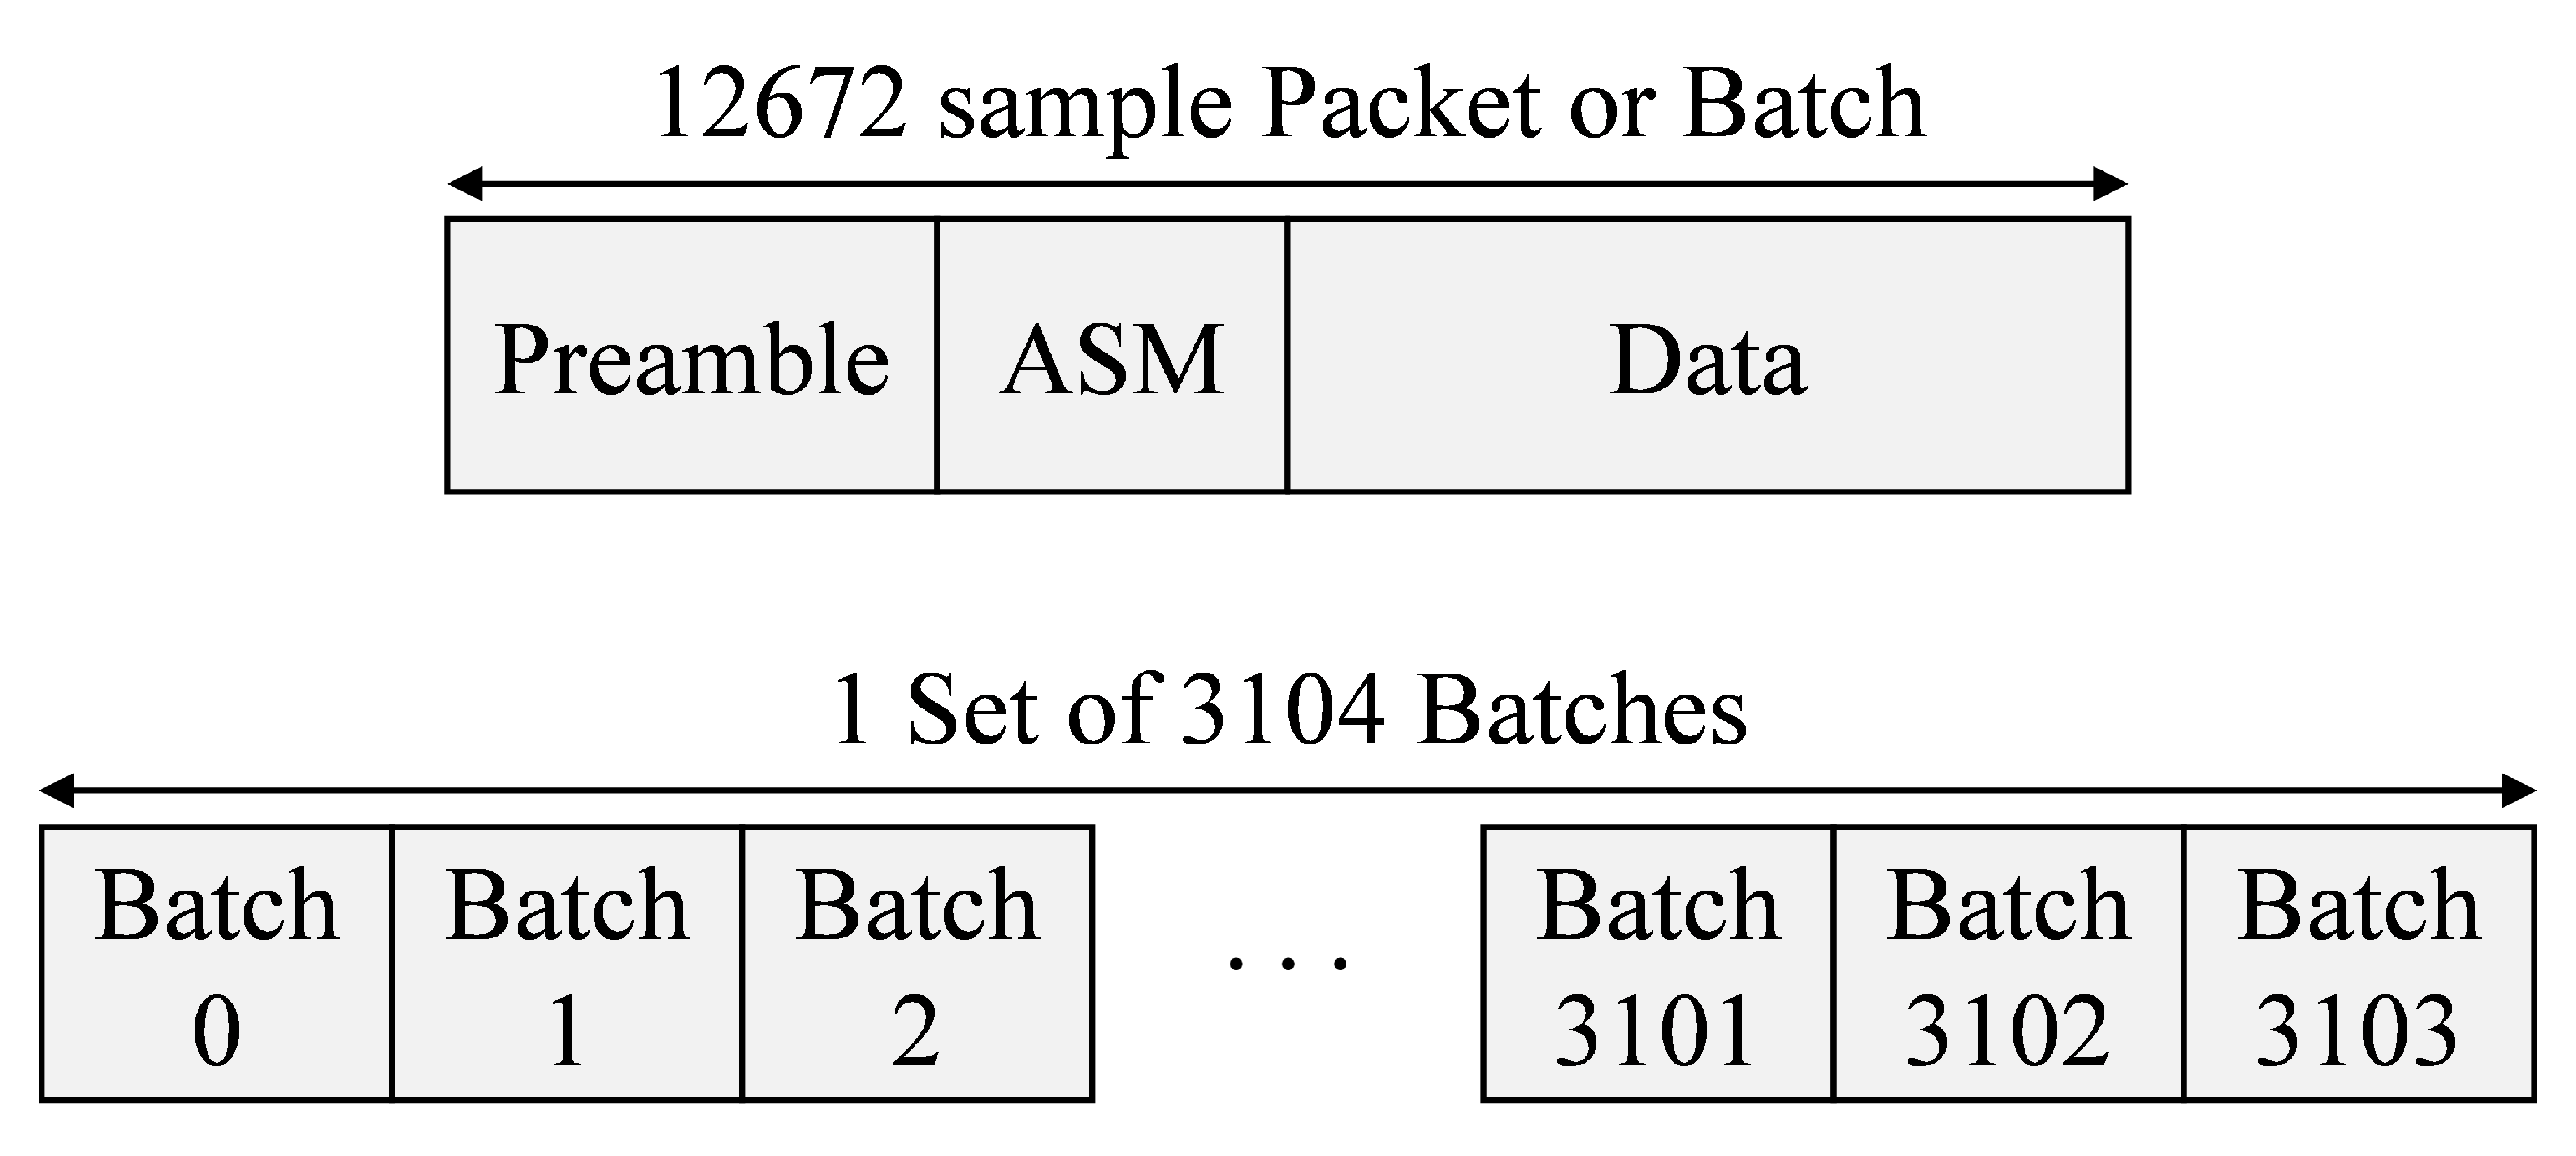
\includegraphics[width=5.94in/100*55]{figures/eq_GPUimplementation/packet_batch_set.pdf}
	\label{fig:packet_batch_set}
	\caption{Set packet structure.}
\end{figure}

The received samples in this thesis has the iNET packet structure shown in Figure \ref{fig:packet}.
The iNET packet consists of a preamble and ASM periodically inserted into the data stream.
The iNET preamble and ASM bits are inserted every 6144 data bits.
The received signal is sampled at 2 samples/bit, making an $\Lpkt=12672$ sample iNET packet.
The iNET preamble comprises eight repetitions of the 16-bit sequence $\text{CD98}_\text{hex}$ and the ASM field
\begin{equation}
034776C72728950B0_\text{hex}.
\end{equation}
Each 16-bit sequence $\text{CD98}_\text{hex}$ sampled at two samples/bit are $L_q=32$ samples long.
\begin{figure}
	\centering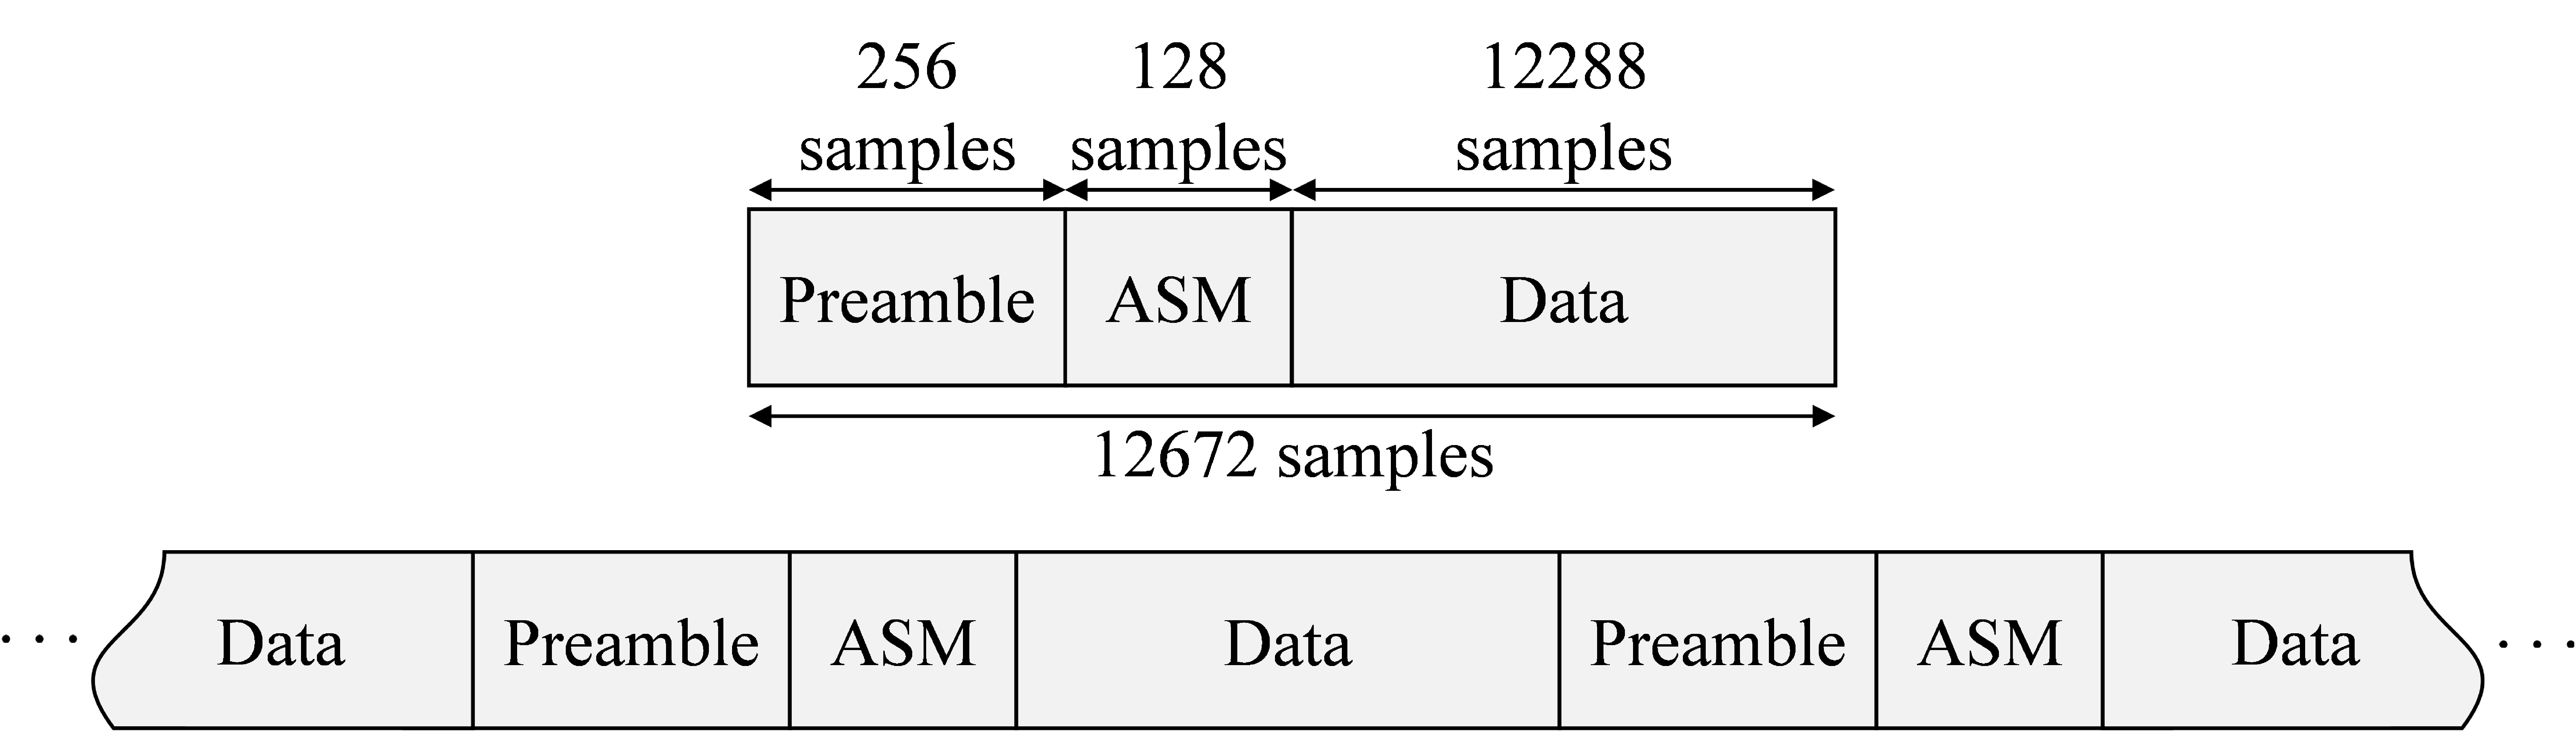
\includegraphics[width=9.47in/100*55]{figures/systemOverview/packetStructure.pdf}
	\label{fig:packet}
	\caption{The iNET packet structure.}
\end{figure}


%\section{Batched Convolution}
%Chapter \ref{chap:gpu} delved into comparing a single convolution in CPUs and GPUs in the time domain or frequency domain.
%As talked about in Chapter blah, system overview, We dont only have a packet or batch, we have $3104$ packets or batches.
%When we perform convolution we convolve $3104$ signals with $3104$ filters.
%So...
%How does the problem change?
%Obviously doing batched convolution in a CPU will not be feasible and wont be considered.
%
%Lets stay in GPU land.
%Should we do convolution in the time domain or the frequency domain?
%Are there draw backs to staying in the time domain? 
%If we do convolution in the time domain, should we use shared memory?
%Are there draw backs for going to the frequency domain? 
%
%Get timing of convolution in the time domain global, time domain shared, time domain frequency.
%
%There is one very important thing we have over looked...
%We are doing just one convolution...we are doing two.
%We have to convolve with the equalizer AND the numerically optimized detection filter $\mathbf{h}_{NO}$.
%If we stay in the time domain, we have to do two cascaded convolutions.
%Two convolutions takes...twice the time....
%If we go to the frequency domain, the point to point or hadamard product is done with 3 inputs rather than 2.
%Convolving with 2 inputs vs even 10 inputs is about the same.
%The only required part is performing the FFT on the inputs and performing the $N$ way multiply...
%
%Well, $\mathbf{h}_{NO}$ doesn't change, so we compute the FFT of the detection filter $\mathbf{H}_{NO}$ and store it.
%So doing the convolution requires taking the FFT of 2 vectors $\mathbf{c}$ and $\mathbf{r}$.
%After the hadamard product, the functions independent of how many filters we are convolving with accept for we may have to trip off different parts depending on what we are convolving with.
%
%Optimizing convolution speeds up every equalizer because every equalizer uses convolution...CMA uses convolution twice per iteration. 
%
%Chapter \ref{chap:eq_eq} the equalizer equations were conditioned for GPU implementation.
%This Chapter explains how the equalizers were implemented into GPUs.
%Block diagrams will be a very helpful tool to display how the GPU kernels flow.
%
%CUDA has many functions that are ``batched,'' meaning the GPU can apply the same function to each packet.
%Don't be confused with the term batch. 
%In the PAQ system, a ``batch'' is 1.907 seconds of data or $3103$ or $3104$ packets.
%In CUDA, ``batched'' kernels are GPU kernels that are called $3103$ or $3104$ times to run on each iNET packet.
%One could say ``The batched kernel runs on a batch of data by processing $3103$ or $3104$ packets.'' 
%The CUDA number of batches is how many iNET packets are being processed.
%
%This sections explains how each equalizer is computed and how the ``numerically optimized'' $H_\text{NO}$ detection filter is applied in each case \cite[Fig. 3]{perrins:2013}.

